\section{Results}
\label{sec:results}

Unless noted otherwise, JevBench numbers follow the disclosures of \Cref{sec:experiments:jevbench}
(public 231-id subset, not a ranked entry, probabilities conditioned on non-$\nullsym$); ``majority/chance''
baselines on that split are .311 standard / .284 easy / .336 hard. Three runs remain in flight at the time
of writing (\texttt{ts1b\_semif}, \texttt{tl1b\_semif}, \texttt{tl2}, a Qwen3.5-9B checkpoint) and are
omitted rather than reported provisionally; we return to this in \Cref{sec:limitations}.

\subsection{Headline results: the scaling ladder and JevBench}
\label{sec:results:headline}

\Cref{tab:headline} runs the identical recipe (\Cref{sec:method}) at four Qwen3 backbone sizes
(1.7B/4B/8B/14B) and once on Qwen3.5-4B, alongside a frozen zero-shot and a frozen three-shot control at
each size (the base model reading next-token letter logits over the rendered options, no training at all).

\begin{table}[t]
  \centering
  \caption{Scaling ladder: JevBench (public subset), MMLU-Pro among-$K$ accuracy, $\dqsh$ (question-conditioned
  signal relative to a fine-tuned 1.7B teacher's own .102), held-out score NLL, and single-decision latency
  at $K{=}2$ (same-pod, same-build numbers; \Cref{sec:experiments:hardware}). Frozen = zero training, letter
  logits only, 3 exemplars. Trained checkpoints: \texttt{ts1b}/\texttt{tm1b} (released as
  \texttt{typical-small}/\texttt{typical-medium}), \texttt{ladder\_8b}, \texttt{tl1b} (candidate),
  \texttt{tm2} (Qwen3.5-4B, trained, not released).}
  \label{tab:headline}
  \small
  \begin{tabular}{lrrrrrrr}
    \toprule
    Model & JevBench std & JevBench hard & Brier (std/hard) & MMLU-K & $\dqsh$ & score NLL & lat.\ (ms) \\
    \midrule
    Qwen3-1.7B (trained) & .694 & .432 & .40 / .79 & .343 & .127 & 1.01 & 45 \\
    Qwen3-1.7B (frozen, 3-shot) & .528 & .369 & -- & -- & -- & -- & -- \\
    Qwen3-4B (trained) & .806 & .423 & .30 / .77 & .458 & .193 & 1.02 & 57 \\
    Qwen3-4B (frozen, 3-shot) & .778 & .441 & -- & -- & -- & -- & -- \\
    Qwen3-8B (trained) & .667 & .396 & .55 / .83 & .290 & .093 & 1.67 & 70 \\
    Qwen3-8B (frozen, 3-shot) & .556 & .369 & -- & -- & -- & -- & -- \\
    Qwen3-14B (trained, \texttt{tl1b}) & \textbf{.931} & .450 & .18 / .66 & .486 & .235 & \textbf{0.95} & 59 \\
    Qwen3-14B (frozen, 3-shot) & .819 & \textbf{.559} & .30 / .60 & -- & -- & -- & -- \\
    Qwen3.5-4B (trained, \texttt{tm2}) & .861 & \textbf{.495} & .22 / .72 & .429 & .194 & 0.97 & -- \\
    \bottomrule
  \end{tabular}
\end{table}

\begin{figure}[t]
  \centering
  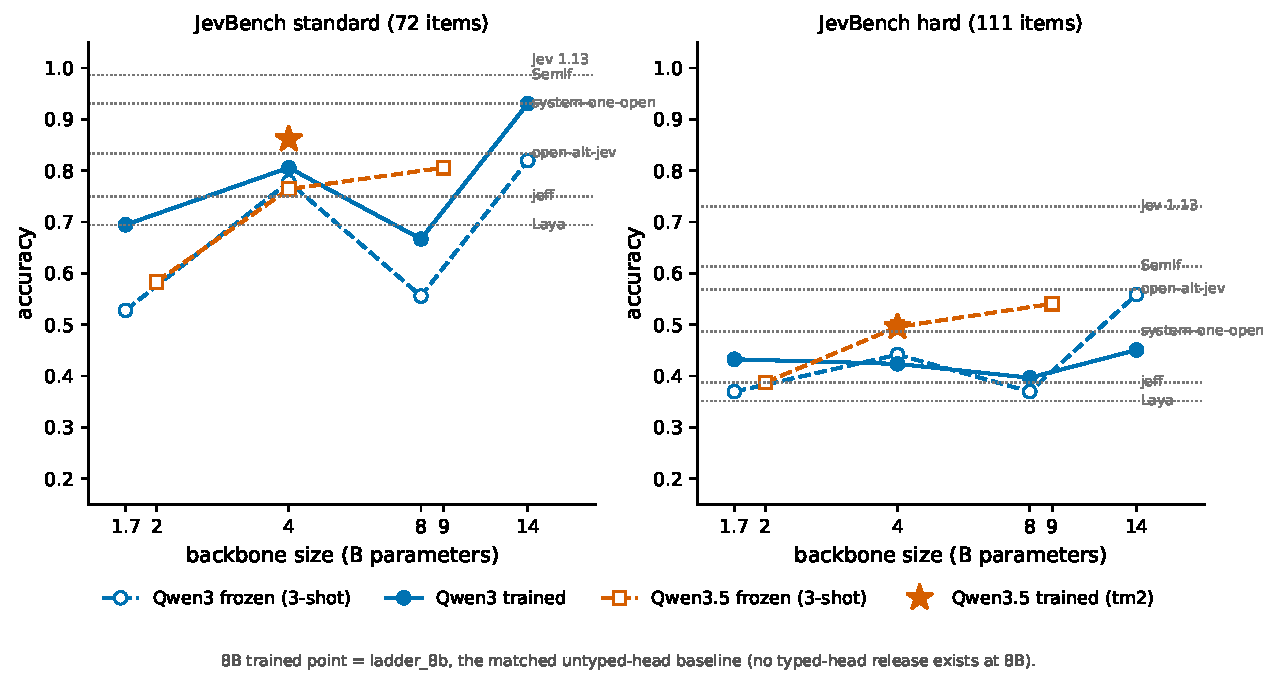
\includegraphics[width=\linewidth]{figures/fig_ladder.pdf}
  \caption{JevBench standard and hard accuracy vs.\ backbone size for Qwen3 (1.7/4/8/14B) and Qwen3.5
  (4B; 2B/9B points from other work's frozen controls where locally available); frozen-with-3-shots dashed,
  trained solid.}
  \label{fig:ladder}
\end{figure}

Two readings anchor the rest of this section. First, standard-tier accuracy, knowledge, and in-distribution
workflow decisions scale close to monotonically with size at roughly constant per-decision latency (45,
57, 59\,ms at $K{=}2$ for 1.7B/4B/14B, \Cref{sec:results:latency}), since a decision's cost is dominated by
the cached-state pass and a short suffix, not backbone depth. Qwen3-8B is an outlier in both frozen and
trained form under the identical recipe; we did not find a tap or learning-rate setting that recovers it
within budget and report it as a checkpoint-specific anomaly (\Cref{sec:limitations}). Second, and this is
the sharper finding: the frozen 14B with three in-context exemplars scores \textbf{.559} on JevBench hard,
above our \emph{trained} 14B's .450 -- training improved standard-tier accuracy and calibration
substantially (Brier .85 $\to$ .66, held-out score NLL 2.87 $\to$ 0.95 after \Cref{sec:results:mixture}--\ref{sec:results:calibration})
while leaving hard-tier \emph{accuracy} below a same-size frozen baseline with no training at all
(\Cref{sec:analysis}).

\subsection{Direct contextual readout replaces the generative interface without losing knowledge}
\label{sec:results:readout}

We compare three non-generative readouts of the same option-in-suffix decision pass: \textbf{N1}, a letter
logit readout (next-token probability over the rendered option letters, the ordinary multiple-choice
interface but read directly rather than generated); \textbf{N2}, a bilinear score between the terminal
state $\hD$ and a candidate-blind semantic embedding of the option text; and \textbf{N3}
(\Cref{sec:method:pass}), a bilinear score between $\hD$ and each option's own contextual hidden state
$\hctx{j}$. \Cref{tab:n1n3} reports the two-seed comparison (identical config, \texttt{seed=0} vs.\
\texttt{seed=1}) at full backbone depth.

\begin{table}[t]
  \centering
  \caption{N1 (letters) vs.\ N3 (direct contextual readout), two seeds, full-depth backbone (28 layers).
  Teacher = a fine-tuned decoder reading options in context. $\dqsh$ is the shuffled-question variant.}
  \label{tab:n1n3}
  \small
  \begin{tabular}{lrrrrr}
    \toprule
    & N1 seed 0 & N1 seed 1 & N3 seed 0 & N3 seed 1 & Teacher \\
    \midrule
    $\dqsh$ (primary) & .114 & .104 & .117 & .094 & .102 \\
    MMLU-Pro among-$K$ & .325 & .318 & .314 & .301 & .310 \\
    SNLI / MNLI / ANLI / BoolQ & .838/.684/.377/.769 & .831/.664/.393/.764 & .863/.752/.431/.737 & .851/.719/.437/.746 & -- \\
    Reorder max $\Delta p$ / IIA $\Delta$log-odds & .165 / .463 & .165 / .443 & .101 / .126 & .109 / .094 & 0 / 0 \\
    \bottomrule
  \end{tabular}
\end{table}

N1 and N3 land within seed noise of each other and of the teacher on $\dqsh$ (N1 mean .109, N3 mean .106,
teacher .102): the direct contextual readout preserves essentially all of the letter interface's
question-conditioned knowledge. It does so with roughly a quarter of the letter interface's order
sensitivity (reorder $\Delta p$ .10--.11 vs.\ .165; independence-of-irrelevant-alternatives violation .09--.13
vs.\ .44--.46) and a consistent evidence-task advantage (SNLI +2, MNLI +6--7, ANLI +4--5 points, both
seeds). \textbf{Depth is the confound that separates the two readouts, not an independent lever.} Reading
the same N3 architecture at the tap-20 truncation used elsewhere in this project rather than the full
28-layer backbone recovers evidence-task accuracy to within 1--3 points of a candidate-blind energy
baseline on every evidence set (and +8 points on CLINC-150) while \emph{keeping} the question-conditioned
signal ($\dqsh$ .118 vs.\ .117 at full depth, 1.16$\times$ the teacher); at the last layer, the same readout
loses evidence accuracy by 5--15 points relative to the energy baseline. Depth is therefore decisive for the
option-conditioned readout in exactly the way it is not decisive for the candidate-blind one
(\Cref{sec:results:candidate-blind}): reading an intermediate layer, not the final one, is required to
recover pretrained evidence reasoning once the options are rendered inside the suffix.

\subsection{The candidate-blind factorization is closed}
\label{sec:results:candidate-blind}

\Cref{sec:method:blind-closure} described the candidate-blind negative result at an intermediate tap.
Because depth turned out to be decisive for the candidate-\emph{aware} readout, we re-ran the strongest
candidate-blind student (eight probes, token-level max-similarity scoring) at full backbone depth to rule
out a tap-depth artifact as the explanation for the earlier null result (full numbers in
\Cref{tab:app-blind-closure}). With the full backbone, $\dqsh$ is $-.008$ (within $\pm .02$ noise of
zero, against .102 for the teacher and $-.026$ for the tap-20 student's choices-only variant), and MMLU-Pro
among-$K$ accuracy \emph{falls} to .147 (from .157 at tap 20), while every evidence task regresses in
exactly the pattern a last-layer tap predicts (SNLI/MNLI/ANLI/BoolQ .881/.807/.462/.712 vs.\ .905/.873/.541/.826
at tap 20: BoolQ $-11$, ANLI $-8$, MNLI $-7$ points). Depth cleanly separates the two readouts: it recovers evidence reasoning for the option-conditioned suffix
and does nothing for a state computed before the candidates are known, at any depth. We take this as the
strongest form of the claim that, under the factorizations and objectives tested here, priors and
calibration compile into a candidate-blind state, but question-conditioned parametric knowledge does not,
independent of tap depth. No further candidate-blind variants were run after this closure.

\subsection{The null: a rendered abstain option is a softmax-dilution bug, not an abstention property}
\label{sec:results:null}

An early native-choice model rendered a literal ``none of the above'' line as one more option in the
suffix and let it compete for softmax mass. Full numbers for this comparison, on an otherwise identical
checkpoint (same tap, same mixture, same steps), are in \Cref{tab:app-null-fix}. Removing the rendered
$\nullsym$ line and replacing it with a gate computed from permutation-invariant statistics of the
candidate scores fixes the null's $K$-dependent pathology essentially for free: the $K$-sweep of null
AUROC becomes monotone (no collapse at small $K$, no always-abstain at large $K$), MMLU-Pro false-abstain
drops from .692 to .003 with accuracy rising from .133 to .353, CLINC-OOS accuracy/null AUROC rise from
.639/.840 to .798/.973, and Banking77 goes from unusable (.063 accuracy, .924 false-abstain) to .579 --
all with $\dqsh$ unchanged (.118 $\to$ .122) and evidence tasks at the same level as the rendered-line
version. The remaining costs are smaller and specific: intent/topic label spaces with tightly clustered
options lose 2--7 points of accuracy, and order sensitivity rises slightly (reorder $\Delta p$ .077 $\to$
.123), because with no null line the letter position is the only identity signal left in the suffix. This
is the single-model, no-workflow-training candidate that scores .694 standard / .378 hard on JevBench and
is the base for every workflow-trained checkpoint reported below.

\subsection{Training the mixture: family ratio, null augmentation, and the long-state truncation fix}
\label{sec:results:mixture}

Adding rubric-conditioned workflow data ($W$) and an uncertainty corpus ($U$) to the evidence/knowledge
mixture of \Cref{sec:results:null} without adjusting sampling ratios costs evidence accuracy: at $E{:}0.35$,
CLINC-150 falls 11 points and TREC-fine 10 points, driven almost entirely by increased false abstention
(CLINC false-abstain .05 $\to$ .17) rather than lost discrimination (CLINC-K accuracy is unchanged; paired
null AUROC is unchanged). \Cref{tab:mixture} sweeps $E$ from .35 to .50 at fixed $K{+}W$ and adds a null
augmentation ablation ($W{:}0.20$ of workflow rows duplicated with their gold removed, target $\nullsym$).

\begin{table}[t]
  \centering
  \caption{Mixture sweep at 1.7B, matched steps. ``6A'' is the $E{:}0.35/K{:}0.25/W{:}0.40$ point;
  ``e45+null'' adds \texttt{null\_aug W:0.20} to $E{:}0.45/K{:}0.20/W{:}0.35$.}
  \label{tab:mixture}
  \small
  \begin{tabular}{lrrrrr}
    \toprule
    & Base ($E$ only) & 6A & e45 & \textbf{e45+null} & long$_{e45}$ (1024 tok) \\
    \midrule
    CLINC-150 acc / false-abstain & .845/.05 & .734/.17 & .779/.10 & \textbf{.805}/\textbf{.08} & .741/.13 \\
    MMLU-Pro among-$K$ / $\dqsh$ & .353/.122 & .330/.119 & .338/.115 & \textbf{.353}/\textbf{.143} & .329/.116 \\
    Held-out score NLL & -- & 2.03 & 1.52 & 2.04 & \textbf{1.26} \\
    JevBench std / hard & .694/.378 & .750/.387 & \textbf{.833}/.396 & .806/.396 & .806/\textbf{.450} \\
    \bottomrule
  \end{tabular}
\end{table}

Raising $E$ to .45--.50 restores evidence accuracy to within 1 point of the $E$-only base and intent/topic
accuracy to within 3--4 points, with $W$ metrics unchanged within 1--4 points: mixing, not architecture, was
the cause of the evidence regression. Null augmentation of $W$ does what a post-hoc calibration offset
cannot (\Cref{sec:results:calibration}): it lowers false-abstain rates and raises MMLU-Pro accuracy to the
$E$-only base's level with the highest $\dqsh$ of any mixture tested. Training at a longer state window
(1{,}024 tokens, 25\% long-policy rows) recovers the long-state families specifically -- before the
facts-first fix described next, this run's long\_policy score rose from .16 to .37 and multi\_hop from .17
to .28 -- and gives the best soft-target NLLs of the sweep, but at a 4$\times$ smaller batch size, which
confounds length with under-fitting; a full-batch version combining every lever (\texttt{r1\_cand}) is the
basis for the released recipe (\Cref{sec:method:mixture}).

\textbf{The long-state truncation bug} (state-length histogram and the fix's effect on long\_policy
accuracy in \Cref{fig:truncation}, \Cref{app:extra-figures}). The long-state generator originally rendered
supporting facts \emph{after} the request text. At the released 1{,}024-token training window this
truncated away the supporting facts on 98.8\% of long-policy rows (100\% at the 256-token window used
earlier in the project), consistent with -- though not, on its own, proven to cause -- the long\_policy
score of .05 at 14B (\Cref{sec:results:headline}) and .21 at 4B: re-rendering facts-first and adding
\texttt{--drop\_truncated} shipped in the same 14B run as frozen-teacher distillation, a Brier-score term,
calibration-based checkpoint selection, and a longer window itself (\Cref{sec:results:kd}), so no matched
single-variable ablation isolates the truncation fix's individual contribution to the long\_policy gain
reported there; we report it as a diagnosed data defect with a plausible mechanism, not a demonstrated
cause.

\subsection{Typed primitives}
\label{sec:results:typed}

\Cref{tab:typed} compares plain $K$-way Choice against the ordinal-smoothed Score target
(\Cref{eq:ordinal-smooth}, $\tauord{=}0.7$) and against the Bernoulli Noul head
(\Cref{eq:bernoulli-noul}), each a matched fine-tune from the same checkpoint on only that type's rows.

\begin{table}[t]
  \centering
  \caption{Typed primitives vs.\ their $K$-way Choice control, matched fine-tunes.}
  \label{tab:typed}
  \small
  \begin{tabular}{lrr}
    \toprule
    Score & $K$-way Choice & Ordinal-smoothed ($\tauord{=}0.7$) \\
    \midrule
    Held-out urgency: acc / NLL / ECE & .505 / 2.07 / .35 & .508 / \textbf{1.23} / \textbf{.19} \\
    JevBench hard: acc / Brier & .360 / .88 & \textbf{.459} / \textbf{.70} \\
    JevBench ordinal items (12), decisions changed & -- & 0 of 12 \\
    \midrule
    Noul & 2-way Choice & Bernoulli \\
    \midrule
    PagerDuty (floor .792): acc / NLL & .602 / 1.04 & \textbf{.886} / \textbf{.28} \\
    Reversed-label max $|\Delta P(\mathrm{yes})|$ & .55 & \textbf{0} (exact, all sets) \\
    \bottomrule
  \end{tabular}
\end{table}

Ordinal smoothing changes \emph{no} decision on JevBench's 12 ordinal items relative to plain Choice --
identical per-item argmax predictions -- while improving every probability-quality metric (held-out score
NLL 2.07 $\to$ 1.23, ECE .35 $\to$ .19, JevBench hard Brier .88 $\to$ .70 with hard accuracy .360 $\to$
.459), confirming it acts purely as a calibration change to the target distribution rather than an
accuracy intervention. The Bernoulli Noul head is exactly order-invariant by construction, verified as a
literal zero reversed-label swing on every evaluated set (against up to .55 for the $K$-way Choice
rendering of the same yes/no question), and is the first head in this project to clear an untouched
external floor by a wide margin (PagerDuty .602 $\to$ .886 against a .792 floor). Both are additive flags
on the same frozen architecture and routed per row (\Cref{sec:method:typed}); the released recipe trains
with both on.

\subsection{DecisionMix v2 and frozen-teacher distillation}
\label{sec:results:kd}

Adding the DecisionMix v2 hard curriculum (\texttt{data\_wh}) and uncertainty corpus (\texttt{data\_u},
\Cref{sec:experiments:data}) moves held-out rule-grammar generalization sharply within the generator's own
world (held-out family/grammar/style accuracy .48/.51/.49 $\to$ .83/.88/.89; rubric-flip accuracy .48
$\to$ .71) but leaves level-7 compositional items -- the reasoning the generator never produces -- at
chance for every model tested, matching the JevBench hard tier's own
temporal/probability/trade-off items. The uncertainty corpus improves likelihood (ChaosNLI NLL 1.27 $\to$
1.00, typed-decisions NLL 2.06 $\to$ 1.71) while top-1 argmax accuracy on the same sets is flat or slightly
lower -- consistent with soft targets teaching the model to spread probability mass rather than sharpen it.

At 14B, combining the facts-first long-state fix, \texttt{--drop\_truncated}, DecisionMix v2, the typed
heads, calibration-shaped checkpoint selection (\Cref{sec:method:selection}), and \textbf{frozen-teacher
distillation} -- a KL term against the \emph{same} backbone's own frozen three-shot letter distribution,
not a larger or external model -- against the previous-recipe 14B checkpoint gives the largest single-run
swing in probability quality observed in this project (\Cref{tab:tl1b}). These five changes shipped
together in one run, so \Cref{tab:tl1b} is evidence for the bundle, not for any one component; a
matched-seed run with distillation removed (\texttt{tl1b\_nokd}) was designed to isolate the KD term
specifically but had not completed evaluation at the time of writing, and no run isolates the long-state
fix alone (\Cref{sec:method:mixture}).

\begin{table}[t]
  \centering
  \caption{14B: previous recipe vs.\ the long-state fix + frozen-teacher KD (\texttt{tl1b}) vs.\ the frozen
  backbone with three exemplars and no training at all.}
  \label{tab:tl1b}
  \small
  \begin{tabular}{lrrr}
    \toprule
    & Previous recipe & \texttt{tl1b} & Frozen, 3-shot \\
    \midrule
    JevBench std / hard & .875 / .468 & \textbf{.931} / .450 & .819 / \textbf{.559} \\
    JevBench Brier (std / hard) & .17 / .85 & .18 / \textbf{.66} & .30 / .60 \\
    Held-out score NLL & 2.87 & \textbf{0.95} & -- \\
    Typed-decisions NLL & 1.96 & \textbf{1.04} & -- \\
    Long\_policy / multi\_hop (hard subfamilies) & .05 / .44 & .158 / .611 & -- \\
    Level-7 composition & -- & \textbf{.620} & -- \\
    \bottomrule
  \end{tabular}
\end{table}

JevBench standard rises from .875 to .931 -- level with the strongest open sub-4B entry on the public
leaderboard -- with knowledge, NLI, and latency unchanged; held-out score NLL falls from 2.87 (the worst
point on the whole size ladder) to 0.95; long\_policy triples and level-7 composition reaches .620, the
first time any checkpoint in this project is clearly above chance there. Hard-tier \emph{accuracy} does
not move (.468 $\to$ .450, within the noise of $n{=}111$) and remains below the frozen 14B's .559 with
three exemplars, even though hard-tier \emph{Brier} improves past it (.66 vs.\ .60 is close, and every
finer-grained probability metric moves far more than accuracy does). We treat this as the clearest
statement of the project's central open tension and discuss it in \Cref{sec:analysis}.

\subsection{Calibration}
\label{sec:results:calibration}

\begin{figure}[t]
  \centering
  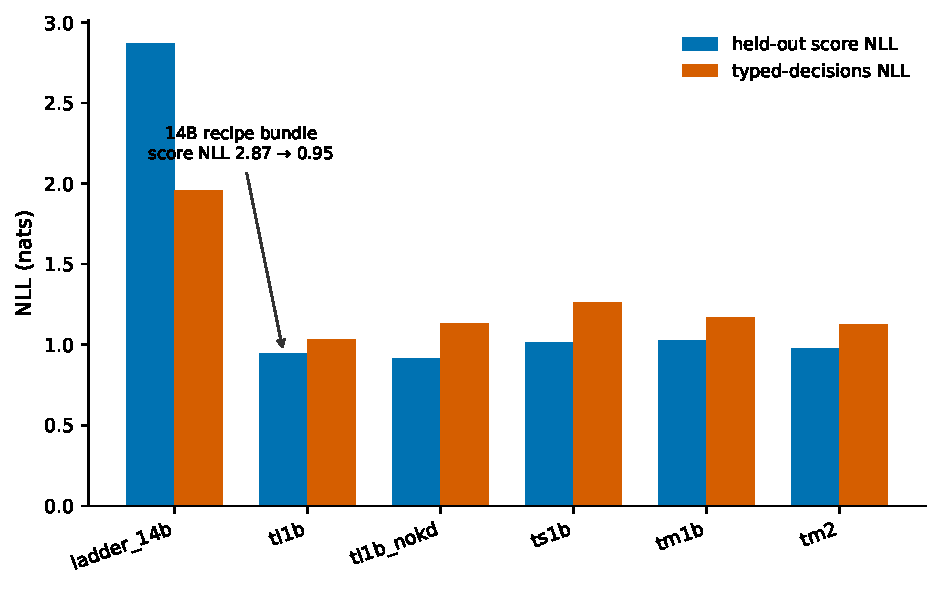
\includegraphics[width=\linewidth]{figures/fig_calibration.pdf}
  \caption{Held-out score NLL and typed-decisions NLL across the calibration-fix sequence
  (\texttt{ladder\_14b} $\to$ \texttt{tl1b}/\texttt{tl1b\_nokd}/\texttt{ts1b}/\texttt{tm1b}/\texttt{tm2}),
  showing the 2.87 $\to$ 0.95 collapse fix.}
  \label{fig:calibration}
\end{figure}

A single global temperature and null-logit offset, fit jointly on held-out soft-target rows, moves in
\emph{opposite} directions for an evidence/knowledge-only checkpoint and a workflow-trained one: for the
former it reduces false abstention and repairs CLINC-150 (false-abstain .053 $\to$ .022); for the latter
the same fitting procedure pushes the offset to $+3.0$, which repairs typed-decisions NLL (1.95 $\to$ 1.19)
but collapses intent/topic coverage to 5--9\%. One global null threshold cannot serve both regimes at once
-- calibration for this class of model needs to be per decision-type or per family, not a single scalar
knob, which is exactly what null augmentation (\Cref{sec:results:mixture}) and per-type target
distributions (\Cref{sec:results:typed}) provide at the data and objective level instead. Selecting
checkpoints on held-out uncertainty-and-curriculum NLL rather than in-distribution loss
(\Cref{sec:method:selection}), combined with training-time Brier regularization rather than only post-hoc
temperature fitting, is the single largest lever on soft-target probability quality found in this project
(\Cref{tab:tl1b}): the standing pattern before this change was that soft-target calibration gets
\emph{worse} with backbone scale under an accuracy-shaped selection criterion (held-out score NLL 2.03 at
1.7B, 2.15 at 4B, 2.87 at 14B); the finding here is that the selection criterion, not backbone capacity,
was the binding constraint.

\subsection{Efficiency}
\label{sec:results:latency}

We report the numbers below as an engineering measurement of this architecture class, not as a benchmarked
systems result: every latency number is a single-stream, Python-level harness with no comparison against
an optimized serving runtime (e.g.\ vLLM or TensorRT-LLM) or a saturated multi-request server, so the
absolute numbers should be read as evidence that a cached-state, no-decode-loop design is viable at these
sizes, not as a tuned lower bound.

\begin{figure}[t]
  \centering
  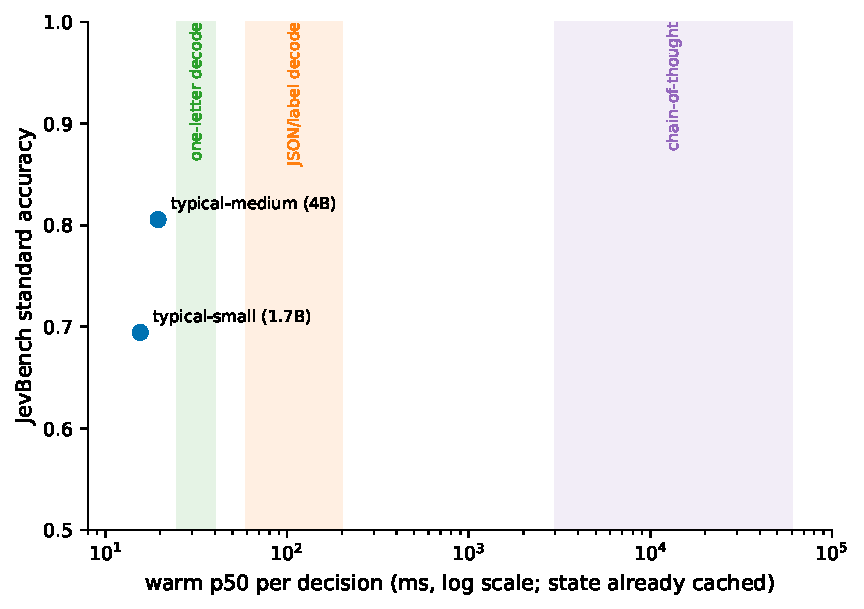
\includegraphics[width=\linewidth]{figures/fig_latency_quality.pdf}
  \caption{JevBench standard accuracy vs.\ measured single-decision latency (ms, log scale) for our
  trained models, with generative-LLM decode-latency comparison bands.}
  \label{fig:latency_quality}
\end{figure}

\textbf{Per-decision latency is close to $K$-independent for bounded candidate sets.} On one H100 (apples-
to-apples, same pod and PyTorch build, 256-token state), a single decision costs 45, 56, and 60\,ms at
1.7B, 4B, and 14B respectively at $K{=}2$, and only rises to 106, 118, and 157\,ms by $K{=}256$ -- an
8$\times$ larger backbone is 1.3$\times$ slower per decision, because the cached state and a short suffix
dominate cost, not backbone depth. Batched marginal cost (cost per query when many queries share one
cached state) scales more steeply with both size and $K$: 2.7\,ms at 1.7B/$K{=}2$ rising to 110\,ms at
14B/$K{=}256$, so the energy-scoring, candidate-blind front end (used to pre-filter very large candidate
sets down to a bounded shortlist before the native readout scores it) matters more at scale, not less.

\textbf{Native choice vs.\ an energy-scoring front end vs.\ a batched log-probability baseline.} At $M{=}256$
queries against one cached 256-token state (transcribed from the run's log; the corresponding
\texttt{bench.json} was lost to an out-of-memory crash, so we report these as a table rather than a
figure), native choice's per-query marginal cost is 1.07, 1.55, 3.38, and 43.8\,ms at $K{=}2, 10, 32, 256$;
a candidate-blind energy-scoring path is flat at $\approx$1\,ms across the same range; and a baseline that
re-runs the backbone once per candidate costs 2.1, 4.6, 12.2, and 101.7\,ms. Native choice is 10--60\%
more expensive than the energy path per query up to $K{\approx}10$ and roughly $3.4\times$ at $K{=}32$ in
this throughput regime, but for a single bounded decision at a time -- the regime most of this paper's
numbers are measured in -- native choice is the cheapest path for $K \le 32$, because its fixed per-call
overhead is lower than the energy path's own front-end cost. The operating rule we adopt is: native choice
directly for bounded sets, energy-scoring $\to$ top-$r$ shortlist $\to$ native choice for very large or
unbounded candidate sets, with $r$ set by the latency budget.

\textbf{Serving-path optimization} (before/after latency by model in \Cref{fig:serving}, \Cref{app:extra-figures}). The public inference package initially deep-copied the entire cached
prefix's key-value tensors on every decision. Replacing this with a zero-copy strided view plus cached
attention masks and position tensors reduced warm per-decision latency from 21--27\,ms to
\textbf{15.5--17\,ms} (\texttt{typical-small}, 1.7B) and \textbf{19--21\,ms} (\texttt{typical-medium}, 4B)
on one H100. We also attempted \texttt{torch.compile}/CUDA-graph capture for a further speedup: a single
fixed input shape reached 8\,ms, but probabilities shifted by up to .1 across the shape buckets the serving
path actually sees, and the mutable key-value cache produced stale-buffer crashes under the standard
capture-and-replay pattern; we reverted this and report it as a rejected optimization. Manual per-bucket
graph capture remains an open path toward $\sim$10\,ms decisions but was not pursued further within budget.
